\chapter{Theory}
\section{The Model Organism/Study Animal}
Euryhaline, osmoconformer, closes valves in periods of exposure to brackish/fresh water (low tide), keeping the saline pallial/mantle fluid as the immediate surrounding environment. Becomes isosmotic with the pallial fluid (Gilles, 1972). In long exposures (> 75 hours) or by puncturing/keeping the valves prised they are forced to pump water, and the hemolymph rapidly conforms to the exterior osmolarity. Short said: is an osmoconformer that behaviorally protects itself from short-term exposures to hypo-osmotic conditions rather than physiologically (Davenport, 1979). Relevant for the osmolarity of buffers/solutions used.

\begin{figure}[h]
    \centering
    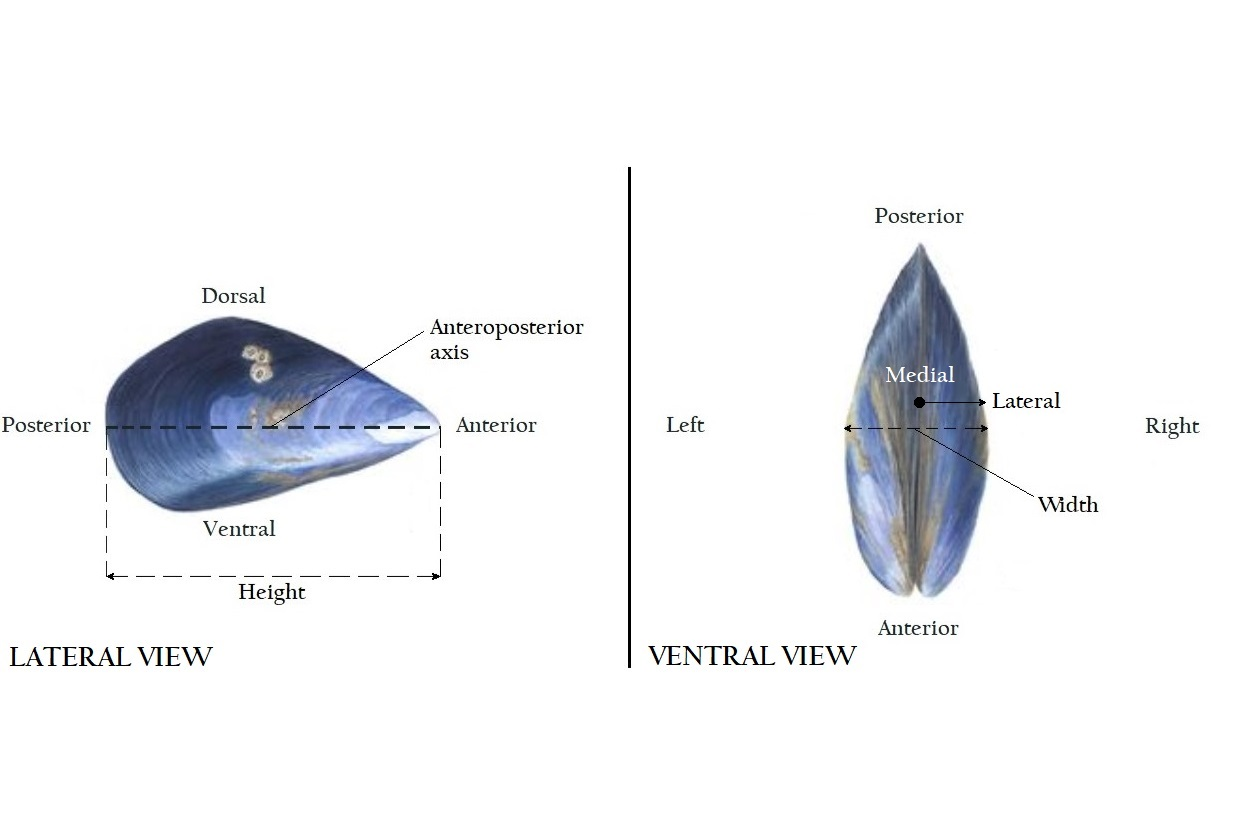
\includegraphics[width=\textwidth]{figures/Anatomy/M_edulis_anatomical_axis_lateral.jpg}
    \caption{The figure caption depends on if it ends up here, or in the material and method. Write when decided. The illustration was adapted from an artistic work by Abby Towne, A. Towne Design with permission.}
    \label{fig:anatomical_axis}
\end{figure}


\subsection{Classification of the haemocyte subpopulations of \emph{M. edulis}}
\label{subsection:haemocyte_classification}
Since the first written account on the subject (\cite{Cuenot1891}, cited in: \cite{Cheng1980}), several authors have devoted their attentions to developing a unifying classification system for the amoebocytic blood cells of bivalve mollusks, more commonly known as haemocytes (\cite{Cheng1980, delaBallina2022}). Belonging to the bivalve familiy \emph{Mytilidae}, the haemocytes of \emph{Mytilus edulis}, \emph{Mytilus galloprovincialis} and several other commercially important species of the genus \emph{Mytilus} have been encompassed by these efforts, creating a substantial pool of literature on the haemocytes of this genus alone. Despite a lack of consensus for any unifying classification system for the haemocytes of this phylum at large, the literature that exists on the haemocytes of \emph{M. edulis} generally agrees on the existence of three distinct subpopulations.

The first effort to classify the haemocytes of \emph{M. edulis} was made by Moore and Lowe (1977). Much like the other attempts to classify bivalve haemocytes at the time, this classification was based on the morphofunctional aspects of these cells - a system that has been extensively reviewed by Hine (1999). Moore and Lowe constructed a simple classification based on static morphological and ultrastructural characteristics of the haemocytes, combined with their phagocytic capacities (\cite{Moore1977}). From routine cytological staining, they identified three haemocyte subpopulations (or cell types): "(1) small basophilic hyaline cells or lymphocytes, (2) larger basophilic hemocytes with varying degrees of irregular cytoplasmic granulation and vacuolation, and (3) eosinophilic granular haemocytes or granulocytes" (\cite{Moore1977}). The small basophilic cells (4-6 \micro m) were generally spherical in outline, had a scant thin rim of basophilic hyaline (read: transparent) cytoplasm and a spherical nucleus - bearing resemblance to vertebrate lymphocytes. The larger granular basophils (7-10 \micro m) displayed less intense basophilic cytoplasm, lower nuclear:cytoplasmic (N:C) ratios and more irregularly shaped nuclei. The eosinophilic granulocytes were the largest cell type identified (7-12 \micro m). They had a regular spherical appearance, further characterized by a small round nucleus, low N:C ratio, and a cytoplasm filled with spherical eosinophilic granules (0.5-1.0 \micro m).

Electron micrographs confirmed the existence of three ultrastructurally distinct morphologies. Except for a few mitochondria, the lymphocyte-like cells contained a scarcity of organelles and granules. This stood in sharp contrast to the larger granular basophils, which contained Golgi apparatus, phagosomes and smaller granular inclusions - possibly representing primary lysosomes. A phagocytosis assay with experimentally injected carbon particles revealed that both granular cell types displayed phagocytic properties, while the small lymphocyte-like cells did not show any evidence for this capacity. To reflect this functional evidence, the granular basophilic haemocytes were classified as phagocytic macrophages. (\cite{Moore1977})

The morphological and ultrastructural findings of Moore and Lowe (1977) have since been confirmed by several investigators (\cite{Rasmussen1985, Renwartz1990, Pipe1990, Noel1994, Pipe1997, Wootton2003}). From their stand-alone electron microscopical examinations, Pipe and colleagues (1990) made a distinction between granular haemocytes with small (0.2-0.3 \micro m) and large (0.5-1.5 \micro m) granules. By relating the two ultrastructural phenotypes to their cytological staining properties, investigators soon demonstrated that the two cell types corresponded to the basophilic and eosinophilic granular haemocytes of Moore and Lowe (\cite{Pipe1990, Noel1994}). Thus, if reduced to it's static morphological criteria, Moore and Lowe's classification of \emph{M. edulis} haemocytes coincides with the original system of Cúenot (1891). This system generally recognized three types of haemocytes in bivalves: "(1) finely granular haemocytes, (2) coarsely granular haemocytes and (3) cells with very little cytoplasm surrounding the nucleus" (\cite{Cheng1984}). 

Leaning towards a phylum-wide two-categorical classification (hyalinocytes and granulocytes), Cheng (1981) argued that a distinction between the basophillic and eosinophilic granulocytes of \emph{M. edulis} was artificial, as he saw them as being immature and mature stages of the same cell type (granulocytes), respectively. From observations of what resembled intermediate stages between the lymphocyte-like and larger basophilic cells, Moore and Lowe (1977) had argued that the basophilic cells constituted an ontogenic developmental series, with the larger phagocytic macrophages representing the final stage of differentiation. This was further supported by observations of lymphocyte-like cells with mitotic figures, suggesting that it could be the stem cell of this lineage (\cite{Moore1977}). Since a few smaller eosinophilic granulocytes (5-7 \micro m) were observed in their sections, the eosinophilic granulocytes were believed to represent a distinct growth series.

As noted by Cheng (1984), this theory was not based on direct evidence, but consisted mainly of interpretive evaluations of morphological findings. The classification bivalve haemocytes should ideally be constructed on the basis of their ontogeny. However, the mapping of ontogenic lineages has been tempered by the lack availible molecular databases, no one unifying model species, combined with uncertainty regarding the hematompoietic tissue(s) and processes of bivalves (\cite{Hine1999, Smith2016, Pila2016, delaBallina2022}). With no real ontogenic evidence to work with, a careful assessment of the availible morphological data may represent a better alternative than founding the classification solely on biochemistry and function (\cite{Hine1999}). 

Almost two decades after flow cytometers became commercially availible in the 1970s (\cite{Shapiro2004}), the application of these instruments started to gain traction within the field of invertebrate immunopathology (\cite{Fisher1988}). Since the traditional characterization of bivalve haemocytes was largely based on morphological criteria such as size, granularity and staining affinities, the simultaneous measurement of forward scatter (FSC, $\approx$ size) and side scatter (SSC, internal complexity $\approx$ granularity) represented a far less subjective approach to their characterization (\cite{AshtonAlcox1998, Allam2002, Mateo2009}).

A detailed flow cytometric characterization of the haemocytes of \emph{M. edulis} was undertaken by Le Foll and colleagues (2010), who were able to distinguish three subpopulations according to their cell diameters (\micro m) and Side Scatter (SSC) (\cite{LeFoll2010}). These comprised one population of small cells (7.14$\pm{0.05}$ \micro m) with low SSC, one population of larger cells (9.97$\pm{0.17}$ \micro m) with intermediate SSC and one population of large cells (10.08$\pm{0.24}$ \micro m) with high SSC. By running haemocytes stained with eosin - which is fluorescent in the green/yellow spectrum under blue laser exitation (\cite{Elfer2016, Koegle2020}) - they were able to identify the latter cluster as eosinophilic granulocytes. The use of flow cytometers equipped with cell sorting capabilities simplifies the process of verifying any classification derived from flow cytometric measurements (\cite{Shapiro2004}). However, when extracting cells with known measured characteristics is not possible, the cells to be classified can be separated by other means prior to flow cytometric acquisition.

Realizing that the three cell types of \emph{M. edulis} differed with regard to the size and density of their granules (or the lack thereof), Friebel (1995) and Pipe (1997) managed to physically separate the eosinophilic granulocytes from the two basophilic cell types by density centrifugation (\cite{Friebel1995, Pipe1997}). Dependent on the treatment prior to centrifugation (fixative, staining), this generally resulted in a separation of the whole haemocyte population into three distinct cell-bands. The two basophillic cell types could be isolated from the upper cell band (lowest density), the eosinophilic granulocytes from the lower, while the intermediate fraction often consisted of varying proportions of all three cell types. Accompanied by the rapid growth of flow cytometric applications in invertebrate immunology, the progress made by Friebel (1995) and Pipe (1997) meant that results from functional and biochemical assays could be assigned to specific cell types at a higher throughput. Thus, the unraveling of the roles of individual haemocyte subpopulations really started to pick up speed.

\section{The role of hemocytes}
Functional classification based on phagocytic capacity: Differences in phagocytosis between granulocytes and agranular haemocytes may be related to the type of phagocytosed particles involved, rather than differences in phagocytic ability (Hine, 1999)


Unlike granulocytes and hyalinocytes, precursor cells do not contribute to immune-response mechanisms such as phagocytosis or encapsulation, and they also lack common intracellular enzyme systems associated with host defence. 

Their lack of cytoplasmic organelles seems to preclude a secretory or phagocytic function

Basophilic cytoplasm suggest the presence of free ribosomes and immaturity

Refer to the 1990 study of Pipe when explaining the functions of the cytoplasmic granules.


Hemocytes also (in addition to lung and digestive gland) showed high expression levels (of initiator and executioner caspases), probably due to the role of apoptosis in the defense against pathogens. Because bivalves are highly susceptible to climate changes, pollutants and pathogens, it  could be suggested that a strong apoptotic process may be necessary to ensure body homeostasis. (Romero, 2011). See page 11 of (New Insights into the Apoptotic Process in Mollusks: Characterization of Caspase Genes in Mytilus galloprovincialis) for greater detail and references.

\section{Bivalve hemocytes as \emph{in vivo} and \emph{in vitro} model systems}
Used as membrane integrity model system. "Since their membranes are susceptible to being destabilised by different stressors, this feature has been frequently used as a biomarker to monitor pollution and animal health (reviewed in Moore et al. 2004, 2006)." From "Changes induced by two strains of Vibrio splendidus in haemocyte subpopulations of Mya arenaria, detected by flow cytometry with LysoTracker" (Mateo, 2009), DOI: 10.3354/dao02121 

Introduce ToPro-3, Calcein AM (Calcein acetoxymethyl) and Apo-15 (\cite{Barth2020}) and their principle of staining, i.e., dye exclusion, cell-permeable (non-specific esterase substrate) and binding to phosphatidyl serine externalized during programmed cell death.

Calcein AM is an electrically neutral molecule, which can easily penetrate cells through diffusion. After acetoxymethyl ester hydrolysis, the negatively charged Calcein molecules are trapped within the cell.

Theory behind Annexin-V/Apo-15: Annexin V
has affinity for phosphatidylserine, which is externalized to the
outer layer of the plasma membrane in the earlier stages of apoptosis. Annexin V also binds internal phosphatidylserine in permeable membranes, i.e. dead cells. Thus, dead cells are Apo-15+ ToPro3+, while the early apoptotiv cells are only Apo15+.

The total hemocyte count (THC) decreased by 66\% after a bacterial injection \cite{Parisi2008}. This could actually be to hemocyte aggregation in response to the needle injection itself.